\newpage
\thispagestyle{empty}
\phantomsection
\addtotoc{Introduction}

\begin{center}\huge \textbf{Introduction}\end{center}

The exponential growth of data volume has propelled the evolution of multi-gigabit 
data transmission in both wireless and wireline communications. This demand is further 
accelerated by the rapid ascent of Artificial Intelligence (AI) and Machine Learning 
(ML) workloads. The training of Large Language Models (LLMs) requires massive datasets 
to be moved between distributed computing nodes with minimal latency. Consequently, 
the ``I/O Wall''---the bottleneck formed by limited interconnect bandwidth---has become 
a critical hurdle \cite{9269409}. High-speed serial links are no longer just a 
communication medium; they are the lifeline of modern hyperscale data centers.

To address these bandwidth-hungry applications, the industry is pushing for higher data 
rates, transitioning from 32~GT/s to 64~GT/s and beyond. This shift necessitates robust 
equalization and signal integrity measures to recover data over lossy channels, which is 
the primary focus of this thesis.

% ==================================================
% PART 1: TRANSMITTER
% ==================================================
\section*{Transmitter Overview}

The transmitter (TX) data path consists of three primary blocks: the \textbf{Clocking 
Network}, the \textbf{High-Speed Serializer (MUX)}, and the \textbf{Line Driver}. Each 
block plays a critical role in generating a clean, high-integrity serial bitstream that 
meets the stringent PCIe Gen~6 electrical specifications.

\subsection*{PCIe Standards Overview}

\subsubsection*{Historical Evolution: From Parallel to Serial}
For decades, the dominant paradigm for connecting peripheral devices to the CPU was the 
parallel bus architecture, where multiple data bits were transmitted simultaneously across 
parallel wires synchronized to a single clock. Early systems relied on the Peripheral 
Component Interconnect (PCI) bus, transferring 32 or 64 bits simultaneously. While 
effective at low speeds, parallel buses suffer from clock skew and crosstalk that make 
synchronization impossible at gigahertz frequencies, necessitating the shift to 
high-speed serial communications.

PCI Express (PCIe) abandoned the parallel bus in favor of point-to-point serial links. 
By embedding the clock within the data stream via Clock and Data Recovery (CDR), PCIe 
eliminated clock skew issues, enabling scalable frequency increases from Gen~1 
(2.5~GT/s) to Gen~6 (64~GT/s). Today, PCIe is the industry standard for connecting 
GPUs, network adapters, and storage drives---the workhorse of data center communication 
driven by AI and Generative AI workloads.

\begin{figure}[H]
    \centering
    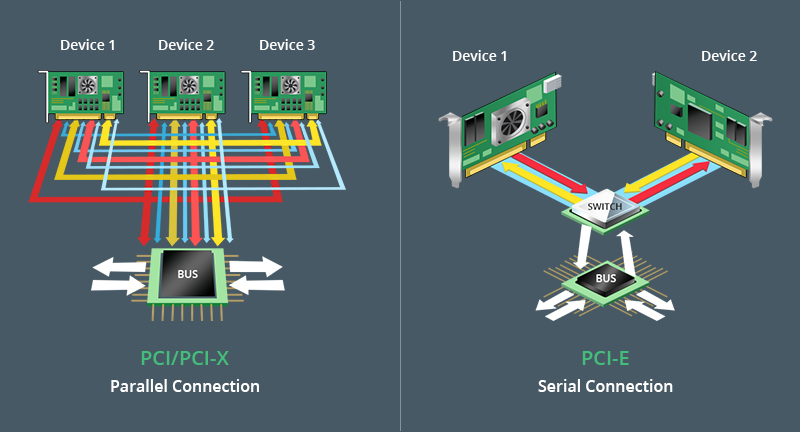
\includegraphics[width=0.5\textwidth]{img/Termination_VGA_img/pcivpcie.png}
    \caption[PCI vs.\ PCIe Architecture]{Evolution of Bus Architectures: Transition 
    from parallel shared-bus PCI topology to high-speed point-to-point serial PCIe 
    links.}
    \label{fig:pci_vs_pcie}
\end{figure}

The PCIe architecture is structured as a three-layer protocol:
\begin{enumerate}
    \item \textbf{Transaction Layer}: Handles TLP assembly, flow control, and reliable 
    packet delivery.
    \item \textbf{Data Link Layer}: Ensures data integrity via LCRC error detection and 
    ACK/NAK re-transmission.
    \item \textbf{Physical Layer (PHY)}: The focus of this thesis---responsible for 
    electrical signaling, serialization, deserialization, and clock recovery.
\end{enumerate}

The standard has evolved through successive generations by advancing modulation and 
encoding techniques:

\textbf{Gen 1.0--2.0 (2.5--5.0~GT/s):} NRZ signaling with 8b/10b encoding, 
introducing a 20\% bandwidth overhead.

\textbf{Gen 3.0--5.0 (8.0--32.0~GT/s):} NRZ signaling with 128b/130b encoding, 
reducing overhead to $\approx$1.5\%.

\textbf{Gen 6.0 (64.0~GT/s):} A revolutionary shift to 4-level Pulse Amplitude 
Modulation (PAM4), transmitting 2~bits per UI and doubling throughput while maintaining 
the same 16~GHz Nyquist frequency as Gen~5. Lightweight Forward Error Correction (FEC) 
and FLIT encoding are mandated to compensate for PAM4's reduced SNR.

\begin{table}[htbp]
    \centering
    \caption{Comparative Analysis of PCIe Generations 3.0--6.0}
    \label{tab:pcie_comparison}
    \begin{tabular}{|l|l|l|l|l|}
        \hline
        \textbf{Feature} & \textbf{PCIe 3.0} & \textbf{PCIe 4.0} & \textbf{PCIe 5.0} 
        & \textbf{PCIe 6.0} \\ \hline
        \textbf{Data Rate}     & 8.0~GT/s  & 16.0~GT/s & 32.0~GT/s & \textbf{64.0~GT/s} \\ \hline
        \textbf{Nyquist Freq}  & 4~GHz     & 8~GHz     & 16~GHz    & \textbf{16~GHz}    \\ \hline
        \textbf{Encoding}      & 128b/130b & 128b/130b & 128b/130b & \textbf{1b/1b FLIT}\\ \hline
        \textbf{Signaling}     & NRZ       & NRZ       & NRZ       & \textbf{PAM4}      \\ \hline
        \textbf{Unit Interval} & 125~ps    & 62.5~ps   & 31.25~ps  & \textbf{31.25~ps}  \\ \hline
        \textbf{Channel Loss}  & 20~dB     & 28~dB     & 36~dB     & \textbf{32~dB}     \\ \hline
    \end{tabular}
\end{table}

\subsection*{GF 22nm FD-SOI Technology}

The transmitter is implemented in GlobalFoundries 22~nm Fully-Depleted 
Silicon-on-Insulator (GF22FDX) technology, selected for its high-speed performance, 
low power consumption, and body-biasing flexibility.

\subsubsection*{Planar MOSFET vs.\ SOI}
\begin{itemize}
    \item \textbf{Electrostatic Control}: SOI provides superior gate control, yielding 
    a subthreshold slope of $S \approx 75$--$85\,$mV/decade vs.\ $\approx 90\,$mV/decade 
    for Bulk CMOS.
    \item \textbf{Parasitic Capacitance}: The insulating buried oxide eliminates 
    source/drain-to-body junction capacitances, enabling higher switching speeds and 
    lower dynamic power.
    \item \textbf{Mobility}: The ultra-thin silicon body requires no heavy channel 
    doping, preserving carrier mobility.
    \item \textbf{Reliability}: SOI is inherently immune to latch-up, though it 
    introduces self-heating due to the low thermal conductivity of the buried oxide.
\end{itemize}

\begin{table}[htbp]
    \centering
    \caption{Key Performance Metrics: Bulk Planar vs.\ SOI}
    \label{tab:bulk_vs_soi}
    \begin{tabular}{lll}
        \toprule
        \textbf{Metric} & \textbf{Bulk Planar MOSFET} & \textbf{SOI} \\
        \midrule
        Substrate           & Semiconductor (p-sub)  & Insulator ($\mathrm{SiO_2}$) \\
        Leakage Control     & Heavy doping required  & Fully depleted channel \\
        Parasitic Cap.\     & High (Junction)        & Eliminated (Body-to-S/D) \\
        Subthreshold Slope  & $\approx 90\,$mV/dec   & $75$--$85\,$mV/dec \\
        Latch-up            & Susceptible            & Immune \\
        \bottomrule
    \end{tabular}
\end{table}

\begin{figure}[H]
    \centering
    \begin{subfigure}{0.48\linewidth}
        \centering
        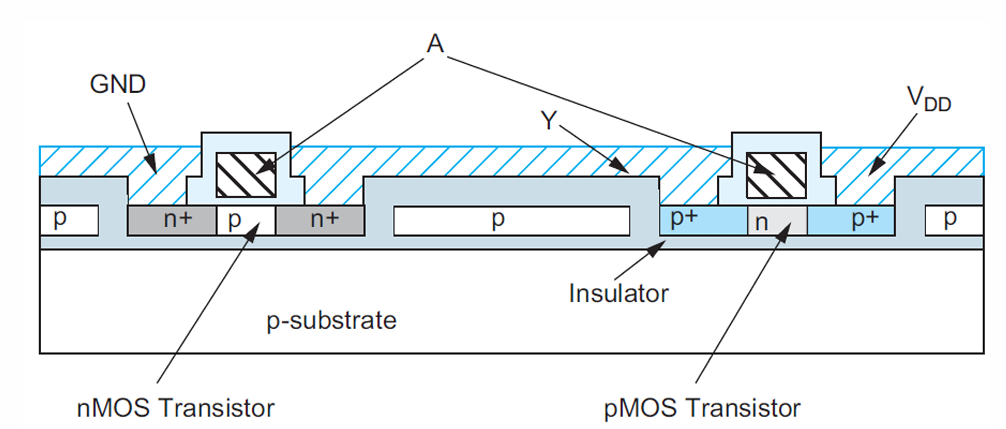
\includegraphics[width=\textwidth]{img/TX_img/soi.png}
        \caption{SOI}
    \end{subfigure}
    \hfill
    \begin{subfigure}{0.5\linewidth}
        \centering
        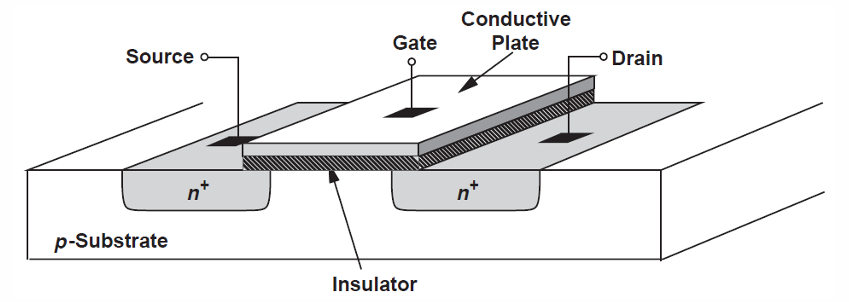
\includegraphics[width=\textwidth]{img/TX_img/bulk.png}
        \caption{Bulk MOSFET}
    \end{subfigure}
    \vspace{0.3cm}
    \caption{Cross-sectional comparison of SOI and Bulk MOSFET device structures.}
    \label{fig:soi_vs_bulk}
\end{figure}

\subsubsection*{Regular Well vs.\ Flip-Well Architecture}

GF22FDX offers two well configurations with distinct body-biasing capabilities:

\textbf{Regular Well:} N-FET in P-well / P-FET in N-well. Optimized for 
\textbf{Reverse Body Biasing (RBB)}, which raises $V_{th}$ to reduce leakage at the 
cost of switching speed. Suited for low-power blocks.

\textbf{Flip-Well:} Reversed doping polarities (N-FET in N-well / P-FET in P-well). 
Enables aggressive \textbf{Forward Body Biasing (FBB)} exceeding 2~V, lowering $V_{th}$ 
and boosting drive current ($I_{on}$) for high-speed operation.

\begin{table}[htbp]
    \centering
    \caption{Regular Well vs.\ Flip-Well in GF22FDX FD-SOI}
    \label{tab:well_comparison}
    \begin{tabular}{lll}
        \toprule
        \textbf{Feature} & \textbf{Regular Well} & \textbf{Flip-Well} \\
        \midrule
        N-FET Placement       & P-well  & N-well \\
        P-FET Placement       & N-well  & P-well \\
        Primary Bias Mode     & RBB     & FBB \\
        Threshold Voltage     & Increased (High $V_{th}$) & Decreased (Low $V_{th}$) \\
        Leakage               & Reduced & Increased \\
        \bottomrule
    \end{tabular}
\end{table}

\begin{figure}[H]
    \centering
    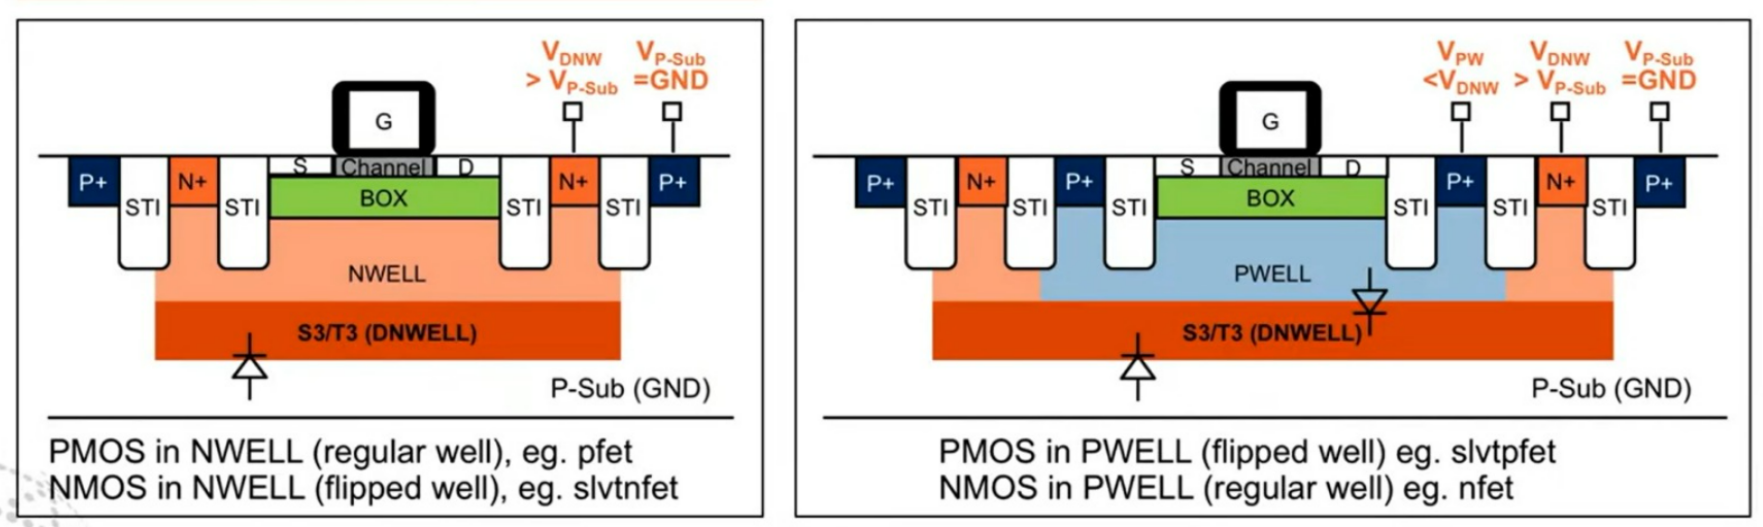
\includegraphics[width=1\textwidth]{img/TX_img/fwell.png}
    \caption{Flip-Well vs.\ Conventional Well in GF22FDX FD-SOI.}
    \label{fig:flip_well}
\end{figure}

% ==================================================
% PART 2: RECEIVER
% ==================================================
\section*{Receiver Overview}

The receiver (RX) data path consists of four primary blocks: the \textbf{Termination 
Network}, the \textbf{Variable Gain Amplifier (VGA)}, the \textbf{Continuous-Time 
Linear Equalizer (CTLE)}, and the \textbf{Decision Feedback Equalizer (DFE)}. Together, 
these blocks reconstruct the attenuated and distorted signal from the channel and recover 
the original data with sufficient margin to meet PCIe Gen~6 BER requirements.

\subsection*{PCIe 6.0 Innovations}

\subsubsection*{PAM4 Signaling}
As shown in Table~\ref{tab:pcie_comparison}, PCIe 6.0 maintains the 16~GHz Nyquist 
frequency of Gen~5 but doubles throughput by adopting PAM4, encoding 2~bits per symbol 
across four distinct voltage levels.

\begin{figure}[H]
    \centering
    \framebox{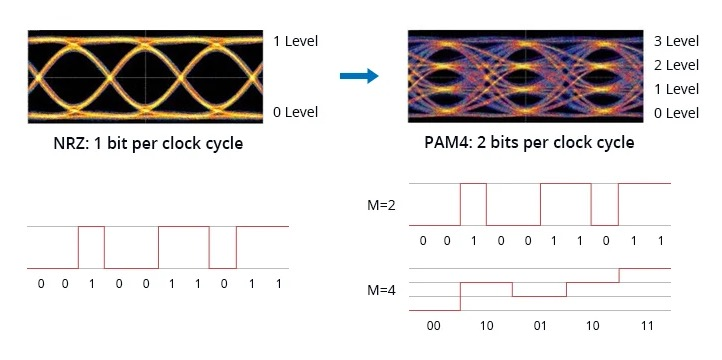
\includegraphics[width=0.7\textwidth]{img/Termination_VGA_img/pam4vnrz.png}}
    \caption[Signaling Comparison]{Comparison of NRZ vs.\ PAM4 Signaling. 
    (\href{https://www.htfwdm.com/info/what-is-pam4-in-400g-53807632.html}{HTF Future})}
    \label{fig:pam4_nrz}
\end{figure}

\subsubsection*{FLIT Encoding}
PCIe 6.0 replaces 128b/130b encoding with \textbf{FLIT Mode}, using fixed 256-byte 
packets with 1b/1b encoding---eliminating encoding overhead entirely. Each FLIT contains:
\begin{itemize}
    \item Transaction Layer Packets (TLP): 236~B
    \item Data Link Packets (DLP): 6~B
    \item Cyclic Redundancy Check (CRC): 8~B
    \item Forward Error Correction (FEC): 6~B
\end{itemize}

\begin{figure}[H]
    \centering
    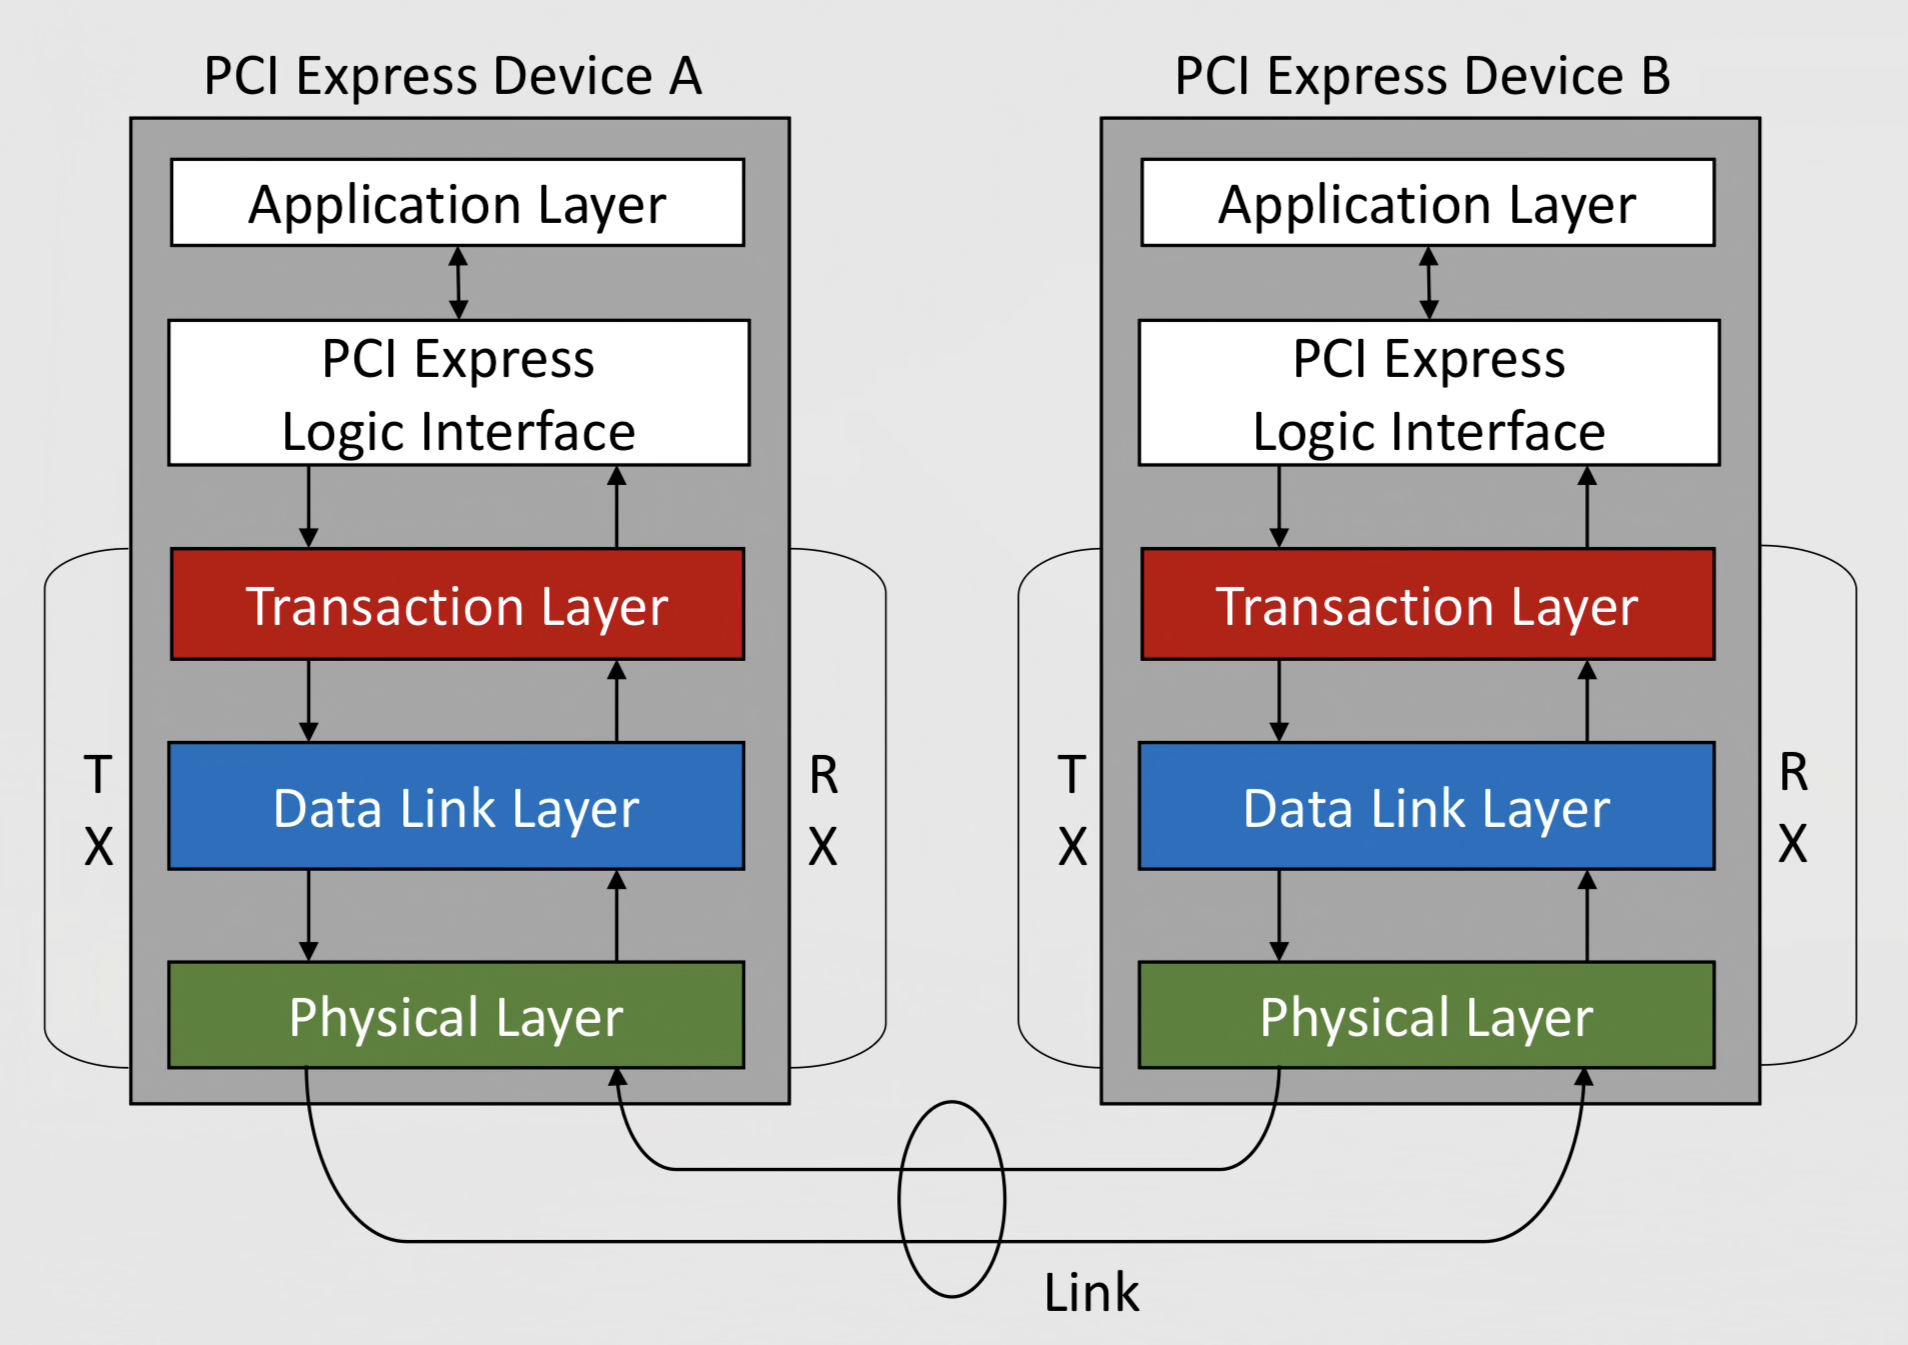
\includegraphics[width=0.5\textwidth]{img/Termination_VGA_img/pciearc.png}
    \caption[PCIe Layer Architecture]{PCIe Protocol Stack and Layer Architecture. 
    (\href{https://www.scribd.com/document/866301752/Introduction-to-PCIe-and-CXL-1746566446}{CERN})}
    \label{fig:pcie_layers}
\end{figure}

\subsubsection*{Forward Error Correction and CRC}
Due to PAM4's reduced SNR (target BER~$< 10^{-6}$ pre-FEC), PCIe 6.0 implements a 
two-stage error handling mechanism within each FLIT:

\begin{enumerate}
    \item \textbf{FEC:} A lightweight, 3-way interleaved FEC corrects burst errors 
    (up to 3 consecutive bytes) caused by DFE error propagation, without requiring 
    re-transmission.
    \item \textbf{CRC:} If FEC correction succeeds, the FLIT is accepted. If errors 
    remain beyond FEC capability, a Link Layer Retry (LLR) is triggered.
\end{enumerate}

This combination maintains a system-level FIT~$< 10^{-9}$---equivalent to prior NRZ 
generations---despite PAM4's inherent signal fragility.